\documentclass{article}

\usepackage{xeCJK}
\setCJKmainfont{SimSun}

\usepackage{listings}
\lstset{breaklines,numbers=left}
\usepackage{hyperref}
\usepackage{pgf}
\usepackage{tikz}
\usetikzlibrary{arrows,shapes,snakes,automata,backgrounds,petri}

\title{FPGA Homework VII\thanks{%
        This homework report is source-opened on
        \href{https://github.com/Qinka/fgpa-homework}{GitHub:Qinka/fpga-homework}.
        Because one of my friend's Java homework, which is also opened on GitHub, was plagiarized by others, I just want declare the my, 李约瀚, copyleft(right) of the report of my homework.
        I, John Lee, is the only writer of this report.
    }}
\author{李约瀚 \\ 14130140331 \\ qinka@live.com \\ me@qinka.pro}

\begin{document}
    \maketitle
    \newpage
    \tableofcontents
    \newpage
    
    \section{Summary}
    \label{sec:summary}
    
    \section{Pratice of State Machine}
    \label{sec:p:sm}
    
    In this part of the homework's report, the pratice is about the state machine.
    The state machine's changing graph, according to the text book, is the figure.
    
    \begin{figure}[h!]
        \centering
        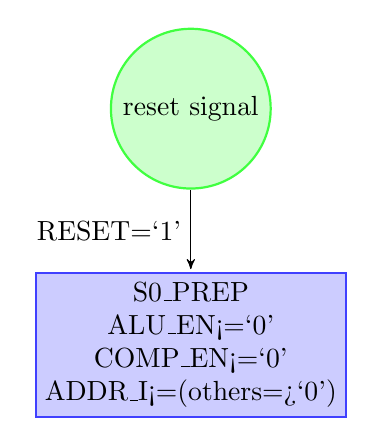
\begin{tikzpicture}[node distance=3cm,>=stealth',bend angle=20,auto]
        \tikzstyle{state}=[rectangle,thick,draw=blue!75,fill=blue!20,minimum size=6mm]
        \tikzstyle{signal}=[circle,thick,draw=green!75,fill=green!20,minimum size=6mm]
        \begin{scope}
        \node[signal](rst){reset signal};
        \node[state,align=center,below of=rst](s1){S0\_PREP \\ ALU\_EN<=`0'\\COMP\_EN<=`0'\\ADDR\_I<=(others=>`0')}
            edge [pre] node{RESET=`1'} (rst);
        \end{scope}
        \end{tikzpicture}
        \caption{Graph}
        \label{fig:sm:changing}
    \end{figure}
    
    
\end{document}